\documentclass[11pt,letterpaper]{article}

\usepackage[margin=0.6in]{geometry}
\usepackage{enumitem}
\usepackage{amsmath}
\usepackage{tikz}
\usetikzlibrary{decorations.pathmorphing, decorations.pathreplacing, calc, arrows.meta}

\pagestyle{empty}
\setlength{\parindent}{0pt}

\begin{document}

\begin{center}
    {\Large \textbf{16.07 Dynamics --- Quiz 6: Spacecraft Dynamics and Thruster Allocation}}
\end{center}

\vspace{4pt}

Name: \rule{3.2in}{0.4pt}

\vspace{10pt}
\begin{enumerate}[label=\textbf{\arabic*.}, leftmargin=*, itemsep=4pt, series=quiz]

\item A single thruster is mounted on a rigid spacecraft at position ${}^{B}\mathbf{r}$ relative to the center of mass $O$. It pushes the spacecraft along the unit vector ${}^{B}\mathbf{d}$ with thrust $u \ge 0$, as shown below. Write the $6\times1$ input Jacobian $\mathbf{B}$ that maps $u$ into the wrench $\bigl[\,{}^{B}\mathbf{F}^T\;\; {}^{B}\boldsymbol{\tau}^T\bigr]^T = \mathbf{B}\,u$, in terms of ${}^{B}\mathbf{r}$ and ${}^{B}\mathbf{d}$.

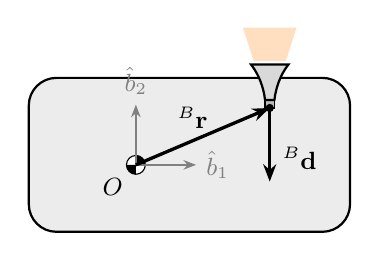
\begin{tikzpicture}[scale=0.85]
    % Spacecraft body
    \filldraw[fill=gray!15, draw=black, thick, rounded corners=10pt] (-1.6,-1.0) rectangle (3.2,1.3);
    % Center of mass
    \filldraw[fill=white] (0,0) circle (4pt);
    \fill (0,0) -- ++(4pt,0) arc (0:90:4pt) -- cycle;
    \fill (0,0) -- ++(-4pt,0) arc (180:270:4pt) -- cycle;
    \node[below left, font=\small] at (-0.05,-0.05) {$O$};
    % Body axes
    \draw[-{Stealth[length=1.6mm]}, thick, gray] (0,0) -- (0.9,0) node[right, font=\small] {$\hat b_1$};
    \draw[-{Stealth[length=1.6mm]}, thick, gray] (0,0) -- (0,0.9) node[above, font=\small] {$\hat b_2$};
    % Thruster location
    \coordinate (P) at (2.0,0.85);
    \draw[-{Stealth[length=2.2mm]}, very thick] (0,0) -- (P);
    \node[font=\small] at (0.85,0.7) {${}^{B}\mathbf{r}$};
    % Thruster bell (exhaust points up, so the force on the spacecraft points down)
    \begin{scope}[shift={(P)}, rotate=90]
        \filldraw[fill=gray!55, draw=black] (0,-0.07) rectangle (0.12,0.07);
        \filldraw[fill=gray!30, draw=black, thick]
            (0.12,0.07) .. controls (0.3,0.09) and (0.5,0.16) .. (0.65,0.28)
            -- (0.65,-0.28) .. controls (0.5,-0.16) and (0.3,-0.09) .. (0.12,-0.07) -- cycle;
        \fill[orange!25] (0.7,0.24) -- (1.2,0.4) -- (1.2,-0.4) -- (0.7,-0.24) -- cycle;
    \end{scope}
    \filldraw (P) circle (1.5pt);
    % Force direction
    \draw[-{Stealth[length=2.2mm]}, very thick] (P) -- ++(0,-1.1);
    \node[font=\small, right] at ($(P)+(0.05,-0.75)$) {${}^{B}\mathbf{d}$};
\end{tikzpicture}
\vspace{0.7in}

\item We wrote the translation dynamics of the Dragon in the inertial (ECI) frame. What if we instead wrote them in the body frame like we had previously in class for the quadrotor, with configuration $\mathbf{q} = \bigl[\,{}^{N}\mathbf{r}^T\;\; \mathbf{a}^T\bigr]^T$ and velocity $\mathbf{v} = \bigl[\,{}^{B}\dot{\mathbf{r}}^T\;\; {}^{B}\boldsymbol{\omega}^T\bigr]^T$? Which terms in the manipulator equation and kinematics would change? Circle them below and write a short explanation.
\begin{center}
\Large
$\dot{\mathbf{q}} \;=\; \mathbf{N}(\mathbf{q})\;\mathbf{v},
\qquad\qquad
\mathbf{M}(\mathbf{q})\;\dot{\mathbf{v}} \;+\; \mathbf{c}(\mathbf{q},\mathbf{v}) \;+\; \mathbf{g}(\mathbf{q}) \;=\; \mathbf{B}(\mathbf{q})\;\mathbf{u}.$
\end{center}
\vspace{1.5in}

\item To allocate thrust, we used the naive pseudoinverse solution $\mathbf{u} = \mathbf{B}^{+}\,{}^{B}\mathbf{w}_{\text{des}}$, and solved the quadratic program
\[
\underset{\mathbf{u}}{\text{minimize}} \;\; \tfrac12\,\mathbf{u}^T\mathbf{u}
\qquad \text{subject to} \qquad
\mathbf{B}\,\mathbf{u} = {}^{B}\mathbf{w}_{\text{des}}, \qquad
0 \le u_i \le u_{\max}.
\]
Recall that the pseudoinverse $\mathbf{B}^{+}\,{}^{B}\mathbf{w}_{\text{des}}$ gives the smallest $\lVert\mathbf{u}\rVert$ that satisfies $\mathbf{B}\,\mathbf{u} = {}^{B}\mathbf{w}_{\text{des}}$. Under what condition will the pseudoinverse solution be the same as the QP solution?
\vspace*{\fill}

\end{enumerate}

\end{document}
